\begin{SCn}
	
\scnsectionheader{\currentname}
	
\scnstartsubstruct

\scnheader{пользовательский интерфейс}
\scnsuperset{командный интерфейс}
\scnsuperset{графический интерфейс}
\scnaddlevel{1}
\scnsuperset{WIMP-интерфейс}
\scnaddlevel{-1}
\scnsuperset{SILK-интерфейс}
\scnaddlevel{1}
\scnidtf{(Speech – речь, Image – образ, Language – язык, Knowledge – знание)}
\scnsuperset{естественно-языковой интерфейс}
\scnaddlevel{1}
\scnsuperset{речевой интерфейс}
\scnaddlevel{-2}

\scnheader{Пользовательский интерфейс}
\scnexplanation{\textbf{Пользовательский интерфейс} -- один из наиболее важных компонентов компьютерной системы. Представляет собой совокупность аппаратных и программных средств, обеспечивающих обмен информацией между пользователем и компьютерной системой.}

\scnheader{Командный пользовательский интерфейс}
\scnexplanation{\textbf{Командный пользовательский интерфейс} -- пользовательский интерфейс, при котором обмен информацией между компьютерной системой и пользователем осуществляется путем написания текстовых инструкций или команд.}

\scnheader{Графический пользовательский интерфейс}
\scnexplanation{\textbf{Графический пользовательский интерфейс} -- пользовательский интерфейс, при котором обмен информацией между компьютерной системой и пользователем осуществляется при помощи графических компонентов компьютерной системы.}

\scnheader{WIMP-интерфейс}
\scnexplanation{\textbf{WIMP-интерфейс} -- пользовательский интерфейс, при котором обмен информацией между компьютерной системой и пользователем осуществляется в форме диалога при помощью окон, меню и других элементов управления.}

\scnheader{SILK-интерфейс}
\scnexplanation{\textbf{SILK-интерфейс} -- пользовательский интерфейс, наиболее приближенный к естественной для человека форме общения. Компьютерная система находит для себя команды, анализируя человеческую речь и находя в ней ключевые фразы. Результат выполнения команд преобразуется в понятную человеку форму, например, в естественно-языковую форму или изображение.}

\scnheader{Естественно-языковой интерфейс}
\scnexplanation{\textbf{Естественно-языковой интерфейс} -- SILK-интерфейс, обмен информацией между компьютерной системой и пользователем в котором происходит за счёт диалога. Диалог ведётся на одном из естественных языков.}

\scnheader{Речевой интерфейс}
\scnexplanation{\textbf{Речевой интерфейс} -- SILK-интерфейс, обмен информацией в котором происходит за счёт диалога, в процессе которого компьютерная система и пользователь общаются с помощью речи. Данный вид интерфейса наиболее приближен к естественному общению между людьми.}

\scnheader{компонент пользовательского интерфейса}
\scnaddlevel{1}
\scnidtf{user interface component}
\scnaddlevel{-1}
	\scnsuperset{компонент пользовательского интерфейса для представления}
	\scnaddlevel{1}
	\scnidtf{presentation user interface component}
	\scnaddlevel{-1}
	\scnaddlevel{1}
		\scnsuperset{компонент вывода}
		\scnaddlevel{1}
		\scnidtf{output}
		\scnaddlevel{-1}
		\scnaddlevel{1}
			\scnsuperset{компонент вывода изображения}
			\scnaddlevel{1}
			\scnidtf{image-output}
			\scnaddlevel{-1}
			\scnsuperset{компонент вывода графической информации}
			\scnaddlevel{1}
			\scnidtf{graphical-output}
			\scnaddlevel{-1}
				\scnaddlevel{1}
				\scnsuperset{диаграмма}
				\scnaddlevel{1}
				\scnidtf{chart}
				\scnaddlevel{-1}
				\scnsuperset{карта}
				\scnaddlevel{1}
				\scnidtf{map}
				\scnaddlevel{-1}
				\scnsuperset{индикатор выполнения} 
				\scnaddlevel{1}
				\scnidtf{progress-bar}
				\scnaddlevel{-1}
				\scnaddlevel{-1}
			\scnsuperset{компонент вывода видео}
			\scnaddlevel{1}
			\scnidtf{video-output}
			\scnaddlevel{-1}
			\scnsuperset{компонент вывода звука}
			\scnaddlevel{1}
			\scnidtf{sound-output}
			\scnaddlevel{-1}
			\scnsuperset{компонент вывода текста}
			\scnaddlevel{1}
			\scnidtf{text-output}
			\scnaddlevel{-1}
				\scnaddlevel{1}
				\scnsuperset{заголовок}
				\scnaddlevel{1}
				\scnidtf{headline}
				\scnaddlevel{-1}
				\scnsuperset{параграф}
				\scnaddlevel{1}
				\scnidtf{paragraph}
				\scnaddlevel{-1}
				\scnsuperset{сообщение}
				\scnaddlevel{1}
				\scnidtf{message}
				\scnaddlevel{-1}
				\scnaddlevel{-2}
	\scnsuperset{декоративный компонент пользовательского интерфейса}
	\scnaddlevel{1}
	\scnidtf{decorative user interface component}
	\scnaddlevel{-1}
		\scnaddlevel{1}
		\scnsuperset{разделитель}
		\scnaddlevel{1}
		\scnidtf{separator}
		\scnaddlevel{-1}
		\scnsuperset{пустое пространство}
		\scnaddlevel{1}
		\scnidtf{blank-space}
		\scnaddlevel{-2}
	\scnsuperset{контейнер}
	\scnidtf{container}
		\scnaddlevel{1}
			\scnsuperset{меню}
			\scnaddlevel{1}
			\scnidtf{menu}
			\scnaddlevel{-1}
			\scnsuperset{строка меню}
			\scnaddlevel{1}
			\scnidtf{menu-bar}
			\scnaddlevel{-1}
			\scnsuperset{панель инструментов}
			\scnaddlevel{1}
			\scnidtf{tool-bar}
			\scnaddlevel{-1}
			\scnsuperset{строка состояния}
			\scnaddlevel{1}
			\scnidtf{status-bar}
			\scnaddlevel{-1}
			\scnsuperset{таблично-строковый контейнер}
			\scnaddlevel{1}
			\scnidtf{table-row-container}
			\scnaddlevel{-1}
			\scnsuperset{списковый контейнер}
			\scnaddlevel{1}
			\scnidtf{list-container}
			\scnaddlevel{-1}
			\scnsuperset{таблично-клеточный контейнер}
			\scnaddlevel{1}
			\scnidtf{table-cell-container}
			\scnaddlevel{-1}
			\scnsuperset{древовидный контейнер}
			\scnaddlevel{1}
			\scnidtf{tree-container}
			\scnaddlevel{-1}
			\scnsuperset{помеченная группа}
			\scnaddlevel{1}
			\scnidtf{labeled-group}
			\scnaddlevel{-1}
			\scnsuperset{панель вкладок}
			\scnaddlevel{1}
			\scnidtf{tab-pane}
			\scnaddlevel{-1}
			\scnsuperset{панель вращения}
			\scnaddlevel{1}
			\scnidtf{spin-pane}
			\scnaddlevel{-1}
			\scnsuperset{узловой контейнер}
			\scnaddlevel{1}
			\scnidtf{tree-node-container}
			\scnaddlevel{-1}
			\scnsuperset{панель прокрутки}
			\scnaddlevel{1}
			\scnidtf{scroll-pane}
			\scnaddlevel{-1}
			\scnsuperset{окно}
			\scnaddlevel{1}
			\scnidtf{window}
			\scnaddlevel{-1}
				\scnaddlevel{1}
				\scnsuperset{модальное окно}
				\scnaddlevel{1}
				\scnidtf{modal-window}
				\scnaddlevel{-1}
				\scnsuperset{немодальное окно}
				\scnaddlevel{1}
				\scnidtf{non-modal-window}
				\scnaddlevel{-4}		
	\scnsuperset{интерактивный компонент пользовательского интерфейса}
	\scnaddlevel{1}
	\scnidtf{interactive user interface component}
	\scnaddlevel{-1}
		\scnaddlevel{1}
		\scnsuperset{компонент ввода данных}
		\scnaddlevel{1}
		\scnidtf{data-input-component}
		\scnaddlevel{-1}
			\scnaddlevel{1}
			\scnsuperset{компонент ввода данных с прямой ответной реакцией}
			\scnaddlevel{1}
			\scnidtf{data-input-component-with-direct-feedback}
			\scnaddlevel{-1}
				\scnaddlevel{1}
				\scnsuperset{компонент ввода текста с прямой ответной реакцией}
				\scnaddlevel{1}
				\scnidtf{text-input-component-with-direct-feedback}
				\scnaddlevel{-1}
					\scnaddlevel{1}
					\scnsuperset{многострочное текстовое поле}
					\scnaddlevel{1}
					\scnidtf{multi-line-text-field}
					\scnaddlevel{-1}
					\scnsuperset{однострочное текстовое поле}
					\scnaddlevel{1}
					\scnidtf{single-line-text-field}
					\scnaddlevel{-1}
					\scnaddlevel{-1}
				\scnsuperset{ползунок}
				\scnaddlevel{1}
				\scnidtf{slider}
				\scnaddlevel{-1}
				\scnsuperset{область рисования}
				\scnaddlevel{1}
				\scnidtf{drawing-area}
				\scnaddlevel{-1}
				\scnsuperset{компонент выбора}
				\scnaddlevel{1}
				\scnidtf{selection-component}
				\scnaddlevel{-1}
					\scnaddlevel{1}
					\scnsuperset{компонент выбора нескольких значений}
					\scnaddlevel{1}
					\scnidtf{selection-component-multiple-values}
					\scnaddlevel{-1}
					\scnsuperset{компонент выбора одного значения}
					\scnaddlevel{1}
					\scnidtf{selection-component-single-values}
					\scnaddlevel{-1}
					\scnaddlevel{-1}
				\scnsuperset{компонент выбора данных}\\
				\scnaddlevel{1}
				\scnidtf{selectable-data-representation}
				\scnaddlevel{-1}	
					\scnaddlevel{1}
					\scnsuperset{флаговая кнопка}
					\scnaddlevel{1}
					\scnidtf{check-box}
					\scnaddlevel{-1}
					\scnsuperset{радиокнопка}
					\scnaddlevel{1}
					\scnidtf{radio-button}
					\scnaddlevel{-1}
					\scnsuperset{переключатель}
					\scnaddlevel{1}
					\scnidtf{toggle-button}
					\scnaddlevel{-1}
					\scnsuperset{выбираемый элемент}
					\scnidtf{selectable-item}
					\scnaddlevel{-2}
			\scnsuperset{компонент ввода данных без прямой ответной реакции}
			\scnaddlevel{1}
			\scnidtf{data-input-component-without-direct-feedback}
			\scnaddlevel{-1}
				\scnaddlevel{1}
				\scnsuperset{кнопка-счётчик}
				\scnaddlevel{1}
				\scnidtf{spin-button}
				\scnaddlevel{-1}
				\scnsuperset{компонент речевого ввода}
				\scnaddlevel{1}
				\scnidtf{speech-input}
				\scnaddlevel{-1}
				\scnsuperset{компонент ввода движений}
				\scnaddlevel{1}
				\scnidtf{motion-input}
				\scnaddlevel{-1}
				\scnaddlevel{-2}
		\scnsuperset{компонент для представления и взаимодействия с пользователем}
		\scnaddlevel{1}
		\scnidtf{presentation-manipulation-component}
		\scnaddlevel{-1}
			\scnaddlevel{1}
			\scnsuperset{активирующий компонент}
			\scnaddlevel{1}
			\scnidtf{activating-component}
			\scnaddlevel{-1}
			\scnsuperset{компонент непрерывной манипуляции}
			\scnaddlevel{1}
			\scnidtf{continuous-manipulation-component}
			\scnaddlevel{-1}
				\scnaddlevel{1}
				\scnsuperset{полоса прокрутки}
				\scnaddlevel{1}
				\scnidtf{scrollbar}
				\scnaddlevel{-1}
				\scnsuperset{компонент редактирования размера}
				\scnaddlevel{1}
				\scnidtf{resizer}
				\scnaddlevel{-1}
				\scnaddlevel{-2}
		\scnsuperset{компонент запроса действий}
		\scnaddlevel{1}
		\scnidtf{operation-trigger-component}
		\scnaddlevel{-1}
			\scnaddlevel{1}
			\scnsuperset{компонент выбора команд}
			\scnaddlevel{1}
			\scnidtf{command-selection-component}
			\scnaddlevel{-1}
				\scnaddlevel{1}
				\scnsuperset{кнопка}
				\scnaddlevel{1}
				\scnidtf{button}
				\scnaddlevel{-1}
				\scnsuperset{пункт меню}
				\scnaddlevel{1}
				\scnidtf{menu-item}
				\scnaddlevel{-1}
				\scnaddlevel{-1}
			\scnsuperset{компонент ввода команд}
			\scnaddlevel{1}
			\scnidtf{command-input-component}
			\scnaddlevel{-1}
			\scnaddlevel{-3}

\scnheader{компонент пользовательского интерфейса для представления}
\scnexplanation{\textbf{компонент пользовательского интерфейса для представления} -- компонент пользовательского интерфейса, не подразумевающий взаимодействия с пользователем.}


\scnheader{компонент вывода}
\scnexplanation{\textbf{компонент вывода} -- компонент пользовательского интерфейса, предназначенный для представления информации.}

\scnheader{компонент вывода изображения}
\scnexplanation{\textbf{компонент вывода изображения} -- компонент пользовательского интерфейса, предназначенный для отображения изображений.}

\scnheader{компонент вывода графической информации}
\scnexplanation{\textbf{компонент вывода графической информации} -- компонент пользовательского интерфейса, предназначенный для представления графической информации.}

\scnheader{диаграмма}
\scnexplanation{\textbf{диаграмма} -- компонент пользовательского интерфейса, предназначенный для отображения графиков.}

\scnheader{карта}
\scnexplanation{\textbf{карта} -- компонент пользовательского интерфейса, предназначенный для отображения карт.}

\scnheader{индикатор выполнения}
\scnexplanation{\textbf{индикатор выполнения} -- компонент пользовательского интерфейса, предназначенный для отображения процента выполнения какой-либо задачи.}

\scnheader{компонент вывода видео}
\scnexplanation{\textbf{компонент вывода видео} -- компонент пользовательского интерфейса, предназначенный для представления видео-информации.}

\scnheader{компонент вывода звука}
\scnexplanation{\textbf{компонент вывода звука} -- компонент пользовательского интерфейса, предназначенный для представления аудио-информации.}

\scnheader{компонент вывода текста}
\scnexplanation{\textbf{компонент вывода текста} -- компонент пользовательского интерфейса, предназначенный для представления текстовой информации.}

\scnheader{заголовок}
\scnexplanation{\textbf{заголовок} -- компонент пользовательского интерфейса, предназначенный для отображения заголовков.}

\scnheader{параграф}
\scnexplanation{\textbf{параграф} -- компонент пользовательского интерфейса, предназначенный для отображения блоков текста. Он отделяется от других блоков пустой строкой или первой строкой с отступом.}

\scnheader{сообщение}
\scnexplanation{\textbf{сообщение} -- компонент пользовательского интерфейса, предназначенный для отображения сообщения.}

\scnheader{декоративный компонент пользовательского интерфейса}
\scnexplanation{\textbf{декоративный компонент пользовательского интерфейса} -- компонент пользовательского интерфейса, предназначенный для стилизации интерфейса.}

\scnheader{контейнер}
\scnexplanation{\textbf{контейнер} -- компонент пользовательского интерфейса, задача которого состоит в размещении набора компонентов, включённых в его состав.
}

\scnheader{меню}
\scnexplanation{\textbf{меню} -- компонент пользовательского интерфейса, содержащий несколько вариантов для выбора пользователем.}

\scnheader{строка меню}
\scnexplanation{\textbf{строка меню} -- горизонтальная полоса , содержащая ярлыки меню. Строка меню предоставляет пользователю место в окне, где можно найти большинство основных функций программы.}

\scnheader{панель инструментов}
\scnexplanation{\textbf{панель инструментов} -- компонент пользовательского интерфейса, на котором размещаются экранные кнопки, значки, меню или другие элементы ввода или вывода.}

\scnheader{строка состояния}
\scnexplanation{\textbf{строка состояния} -- компонент пользовательского интерфейса, предназначенный для отображения информации о текущем состоянии окна.}

\scnheader{списковый контейнер}
\scnexplanation{\textbf{списковый контейнер} -- контейнер, который располагает элементы интерфейса в виде списка.}

\scnheader{таблично-клеточный контейнер}
\scnexplanation{\textbf{таблично-клеточный контейнер} -- контейнер, который располагает элементы интерфейса в виде таблицы.}

\scnheader{древовидный контейнер}
\scnexplanation{\textbf{древовидный контейнер} -- контейнер, который располагает элементы интерфейса в виде дерева.}

\scnheader{панель вкладок}
\scnexplanation{\textbf{панель вкладок} -- контейнер , который может содержать несколько вкладок (секций) внутри, которые могут быть отображены, нажав на вкладке с названием в верхней части панели. Одновременно отображается только одна вкладка.}

\scnheader{панель прокрутки}
\scnexplanation{\textbf{панель прокрутки} -- компонент пользовательского интерфейса, который позволяет пользователю прокручивать его содержимое.}

\scnheader{окно}
\scnexplanation{\textbf{окно} -- обособленная область экрана, содержащая различные элементы пользовательского интерфейса. Окна могут располагаться поверх друг друга.}

\scnheader{модальное окно}
\scnexplanation{\textbf{модальное окно} -- окно, которое блокирует работу пользователя с родительским приложением до тех пор, пока пользователь  окно не закроет.}

\scnheader{немодальное окно}
\scnexplanation{\textbf{немодальное окно} -- окно, которое позволяет перемещать фокус между окном диалога и другой формой без необходимости закрыть окно диалога.}

\scnheader{интерактивный компонент пользовательского интерфейса}
\scnexplanation{\textbf{интерактивный компонент пользовательского интерфейса} -- компонент пользовательского интерфейса, с помощью которого осуществляется взаимодействие с пользователем.}

\scnheader{компонент ввода данных}
\scnexplanation{\textbf{компонент ввода данных} -- компонент пользовательского интерфейса, предназначенный для ввода информации.}

\scnheader{многострочное текстовое поле}
\scnexplanation{\textbf{многострочное текстовое поле} -- поле ввода, которое позволяет работать с несколькими строками текста.}

\scnheader{однострочное текстовое поле}
\scnexplanation{\textbf{однострочное текстовое поле} -- поле ввода, которое позволяет работать только с одной строкой текста.}

\scnheader{ползунок}
\scnexplanation{\textbf{ползунок} -- компонент пользовательского интерфейса, с помощью которого пользователь может установить значение, перемещая индикатор, обычно по горизонтали.}

\scnheader{область рисования}
\scnexplanation{\textbf{область рисования} -- прямоугольная область, которая поддерживает рисование и получение входных данных (щелчки мыши, движение мыши и нажатия клавиш).}

\scnheader{компонент выбора}
\scnexplanation{\textbf{компонент выбора} -- компонент пользовательского интерфейса, предназначенный для выбора.}

\scnheader{компонент выбора нескольких значений}
\scnexplanation{\textbf{компонент выбора нескольких значений} -- компонент выбора, в котором можно выбрать значения для различных свойств.}

\scnheader{компонент выбора одного значения}
\scnexplanation{\textbf{компонент выбора одного значения} -- компонент выбора, в котором можно установить значение только одного свойства.}

\scnheader{компонент выбора данных}
\scnexplanation{\textbf{компонент выбора данных} -- компонент пользовательского интерфейса, который позволяет выбрать отображаемые данные.}

\scnheader{флаговая кнопка}
\scnexplanation{\textbf{флаговая кнопка} -- компонент пользовательского интерфейса, позволяющий пользователю управлять параметром с двумя состояниями — включено и отключено.}

\scnheader{радиокнопка}
\scnexplanation{\textbf{радиокнопка} -- компонент пользовательского интерфейса, который позволяет пользователю выбрать одну опцию из предопределенного набора.}

\scnheader{переключатель}
\scnexplanation{\textbf{переключатель} -- компонент пользовательского интерфейса, который позволяет пользователю переключаться между двумя состояниями.}

\scnheader{выбираемый элемент}
\scnexplanation{\textbf{выбираемый элемент} -- элемент компонента "компонент выбора одного значения".}

\scnheader{кнопка-счетчик}
\scnexplanation{\textbf{кнопка-счетчик} -- компонент пользовательского интерфейса, как правило, ориентированный вертикально, с помощью которого пользователь может изменить значение в прилегающем текстовом поле, щёлкнув на стрелку вверх или вниз, или удерживая стрелку вверх или вниз, в результате чего значение в текстовом поле увеличивается (если нажата стрелка вверх) или уменьшается (если нажата стрелка вниз).}

\scnheader{компонент речевого ввода}
\scnexplanation{\textbf{компонент речевого ввода} -- компонент пользовательского интерфейса для ввода речи.}

\scnheader{компонент ввода движений}
\scnexplanation{\textbf{компонент ввода движений} -- компонент пользовательского интерфейса для ввода движений.}

\scnheader{компонент для представления и взаимодействия с пользователем}
\scnexplanation{\textbf{компонент для представления и взаимодействия с пользователем} -- компонент пользовательского интерфейса, предназначенный для представления информации и взаимодействия с пользователем.}

\scnheader{полоса прокрутки}
\scnexplanation{\textbf{полоса прокрутки} -- компонент пользовательского интерфейса, который используется для отображения информации и элементов интерфейса, больших по размеру, чем используемый для их отображения контейнер.}

\scnheader{редактор размера}
\scnexplanation{\textbf{редактор размера} -- компонент пользовательского интерфейса, с помощью которого можно изменять размер другого компонента.}

\scnheader{компонент запроса действий}
\scnexplanation{\textbf{компонент запроса действий} -- компонент пользовательского интерфейса, который запрашивают пользователя совершить некоторое действие.}

\scnheader{кнопка}
\scnexplanation{\textbf{кнопка} -- компонент пользовательского интерфейса, при нажатии на который происходит программно связанное с этим нажатием действие либо событие.}

\scnheader{пункт меню}
\scnexplanation{\textbf{пункт меню} -- элемент компонента меню.}

\scnheader{Стартовая страница}
\scnrelfrom{иллюстрация}{
\scnfileimage{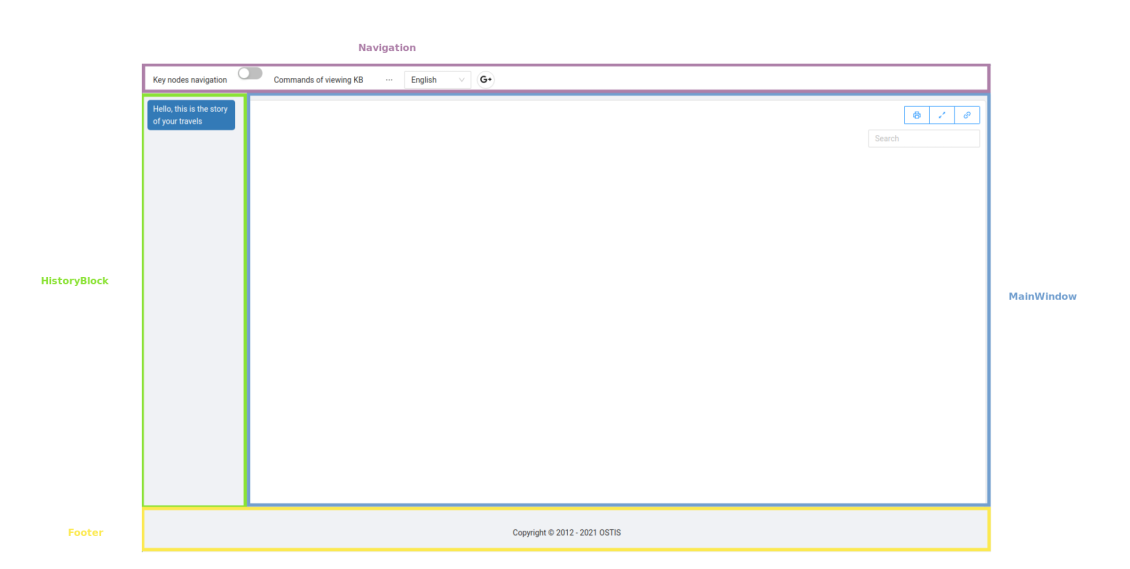
\includegraphics[width=1\linewidth]{figures/sd_ui/startPage.png}}}
\scnaddlevel{1}
\scniselement{окно}
\scnhaselementrole{пример}{\\
\scnrelfromset{декомпозиция}{
Навигация\\
	\scnaddlevel{1}
	\scniselement{неатомарный компонент пользовательского интерфейса}
	\scnrelfromset{декомпозиция}{
	Главное меню\\	
		\scnaddlevel{1}
		\scniselement{меню}
		\scnhaselementrole{пример}{\\
		\scnrelfromset{декомпозиция}{
		Элемент-1\\
			\scnaddlevel{1}
			\scniselement{пункт меню}
			\scnaddlevel{-1}
		;Элемент-2\\
			\scnaddlevel{1}
			\scniselement{пункт меню}
			\scnaddlevel{-1}			
		;Переключение режима\\
			\scnaddlevel{1}
			\scniselement{переключатель}
			\scnaddlevel{-1}
	}
}
	\scnaddlevel{-1}
	;Выбор языка\\
		\scnaddlevel{1}
		\scniselement{компонент выбора одного значения}
		\scnaddlevel{-1}
	;Гугл\\
		\scnaddlevel{1}
		\scniselement{кнопка}
		\scnaddlevel{-1}
	\scnaddlevel{-1}
;Блок истории\\
	\scnaddlevel{1}
	\scniselement{неатомарный компонент пользовательского интерфейса}
	\scnaddlevel{-1}
;Основной блок\\
	\scnaddlevel{1}
	\scniselement{неатомарный компонент пользовательского интерфейса}
	\scnrelfromset{декомпозиция}{
	Главное окно\\
		\scnaddlevel{1}
		\scniselement{окно}
		\scnaddlevel{-1}
	;панель инструментов\\
		\scnaddlevel{1}
\scnhaselementrole{пример}{\\
		\scnrelfromset{декомпозиция}{Кнопка принтера\\
			\scnaddlevel{1}
			\scniselement{кнопка}
			\scnaddlevel{-1}
		;Кнопка со стрелками\\
			\scnaddlevel{1}
			\scniselement{кнопка}
			\scnaddlevel{-1}
		;Кнопка ссылки\\
			\scnaddlevel{1}
			\scniselement{кнопка}
			\scnaddlevel{-1}
		;Поиск\\	
			\scnaddlevel{1}
			\scniselement{однострочное текстовое поле}
			\scnaddlevel{-1}}
	}}
	\scnaddlevel{-1}
	}\scnaddlevel{-1}
;Футер\\
	\scnaddlevel{1}
	\scniselement{неатомарный компонент пользовательского интерфейса}
	\scnaddlevel{-1}
}
}
\scnendstruct \scnendcurrentsectioncomment
\end{SCn}